\documentclass[tikz,border=3pt]{standalone}
\usepackage[utf8]{inputenc}
\usepackage[T1]{fontenc}
\usepackage{lmodern}
\renewcommand{\familydefault}{\sfdefault}
\usepackage{sansmath}\sansmath
\usepackage{chemfig}
\usepackage{pgfplots}\pgfplotsset{compat=1.18,/pgf/number format/use comma,/pgf/number format/1000 sep={.}}
\usetikzlibrary{arrows.meta,calc,positioning,decorations.pathmorphing,patterns}
% paleta del sitio
\definecolor{nar}{HTML}{E8680C}\definecolor{narc}{HTML}{FFB35C}\definecolor{hielo}{HTML}{FFF3E8}
\definecolor{tinta}{HTML}{1D1D1F}\definecolor{gris}{HTML}{6E6E73}\definecolor{lila}{HTML}{7C5CF0}
\definecolor{azul}{HTML}{2F6FD6}\definecolor{menta}{HTML}{17A673}\definecolor{coral}{HTML}{E8342A}
\begin{document}
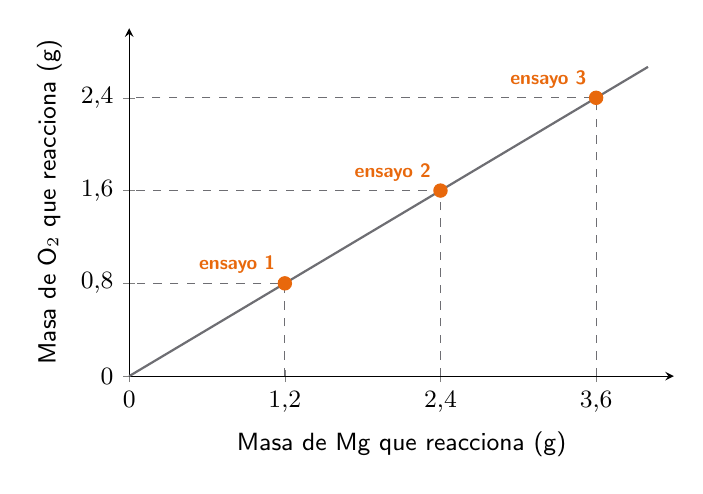
\begin{tikzpicture}[font=\small]
\begin{axis}[width=8.5cm,height=6cm,axis lines=left,xmin=0,xmax=4.2,ymin=0,ymax=3.0,xtick={0,1.2,2.4,3.6},ytick={0,0.8,1.6,2.4},
  xticklabel style={/pgf/number format/fixed,/pgf/number format/precision=1},yticklabel style={/pgf/number format/fixed,/pgf/number format/precision=1},
  xlabel={Masa de Mg que reacciona (g)},ylabel={Masa de O$_2$ que reacciona (g)},clip=false]
\addplot[gris,thick,domain=0:4.0] {2*x/3};
\addplot[only marks,mark=*,mark options={fill=nar,draw=nar,scale=1.2}] coordinates {(1.2,0.8)(2.4,1.6)(3.6,2.4)};
\draw[dashed,gris] (axis cs:1.2,0) -- (axis cs:1.2,0.8) -- (axis cs:0,0.8);
\draw[dashed,gris] (axis cs:2.4,0) -- (axis cs:2.4,1.6) -- (axis cs:0,1.6);
\draw[dashed,gris] (axis cs:3.6,0) -- (axis cs:3.6,2.4) -- (axis cs:0,2.4);
\node[font=\scriptsize\bfseries,text=nar,anchor=south east] at (axis cs:1.2,0.8) {ensayo 1};
\node[font=\scriptsize\bfseries,text=nar,anchor=south east] at (axis cs:2.4,1.6) {ensayo 2};
\node[font=\scriptsize\bfseries,text=nar,anchor=south east] at (axis cs:3.6,2.4) {ensayo 3};
\end{axis}
\end{tikzpicture}
\end{document}
